\chapter{Methodology}

\section{Collecting Data: OONI}

\subsection{Background}
Released under the TOR project in 2012, the Open Observatory of Network Interference (OONI) is a non-profit open-source software project whose goal is to empower decentralized efforts to document internet censorship worldwide \cite{OONIAbout}. The OONI organization openly publishes measurements and provides a public archive of network interference across the globe. This has produced a database of more than 2.6 billion individual tests. \cite{OONIExplorer}

OONI data has been used extensively by third parties both for research and advocacy. Examples include the Freedom on the Net 2024 \cite{freedomhouse2024struggle} report, iMAP reports \cite{ooni2024imap} by Sinar, and Access Now’s annual \#KeepItOn 2023 Report. \cite{accessnow2023keepiton} \cite{ooni2024yearinreview} Based on these high profile endorsements and the wealth of data available, OONI is a perfect tool to measure internet censorship.

\subsection{OONI Probe}
Released in 2017, the OONI Probe is a mobile app and software designed to test internet censorship. Users can install and run this software, contributing to the growing dataset in the OONI database. OONI's mission is to \textit{“ensure a free and open internet by increasing transparency of internet censorship worldwide.”} While no user appears to have faced repercussions from using the OONI probe, this may lead to a false sense of security or incorrect assumptions about anonymity. As emphasized in OONI’s onboarding quiz, probe tests can be visible on the network.

\subsection{Virtual Machine}
In order to gather ground truth, a virtual machine in Israel is used to run OONI command line interface locally. This machine is accessed via SSH. These technologies will be discussed further below. The chosen provider, \textit{interhost.co.il}, has a strong track record regarding data integrity and security; however, further scrutiny is necessary. \cite{interhost} 

These tools were audited for any security and privacy concerns and the results are below. Tools like CloudFlare's TCP reset dashboard \cite{cloudflare_policy_blog} gave further insight on instances of throttling, blocking or otherwise. In order to expand the web connectivity tests included with OONI, resources like Citizen Lab's sensitive domain list were included. \cite{citizenlab_testlists} 

\section{Ground Truth: Ireland \& Israel}
To gather ground truth in Ireland, the OONI probe Command Line Interface was installed and ran over a two week period. Since the CLI is not natively supported on Windows, a Unix-based operating system was flashed onto a Raspberry Pi 5, which served as a dedicated headless testing device. The device was accessed remotely via SSH, enabling the automation and management of tests. 

\begin{figure}
    \centering
    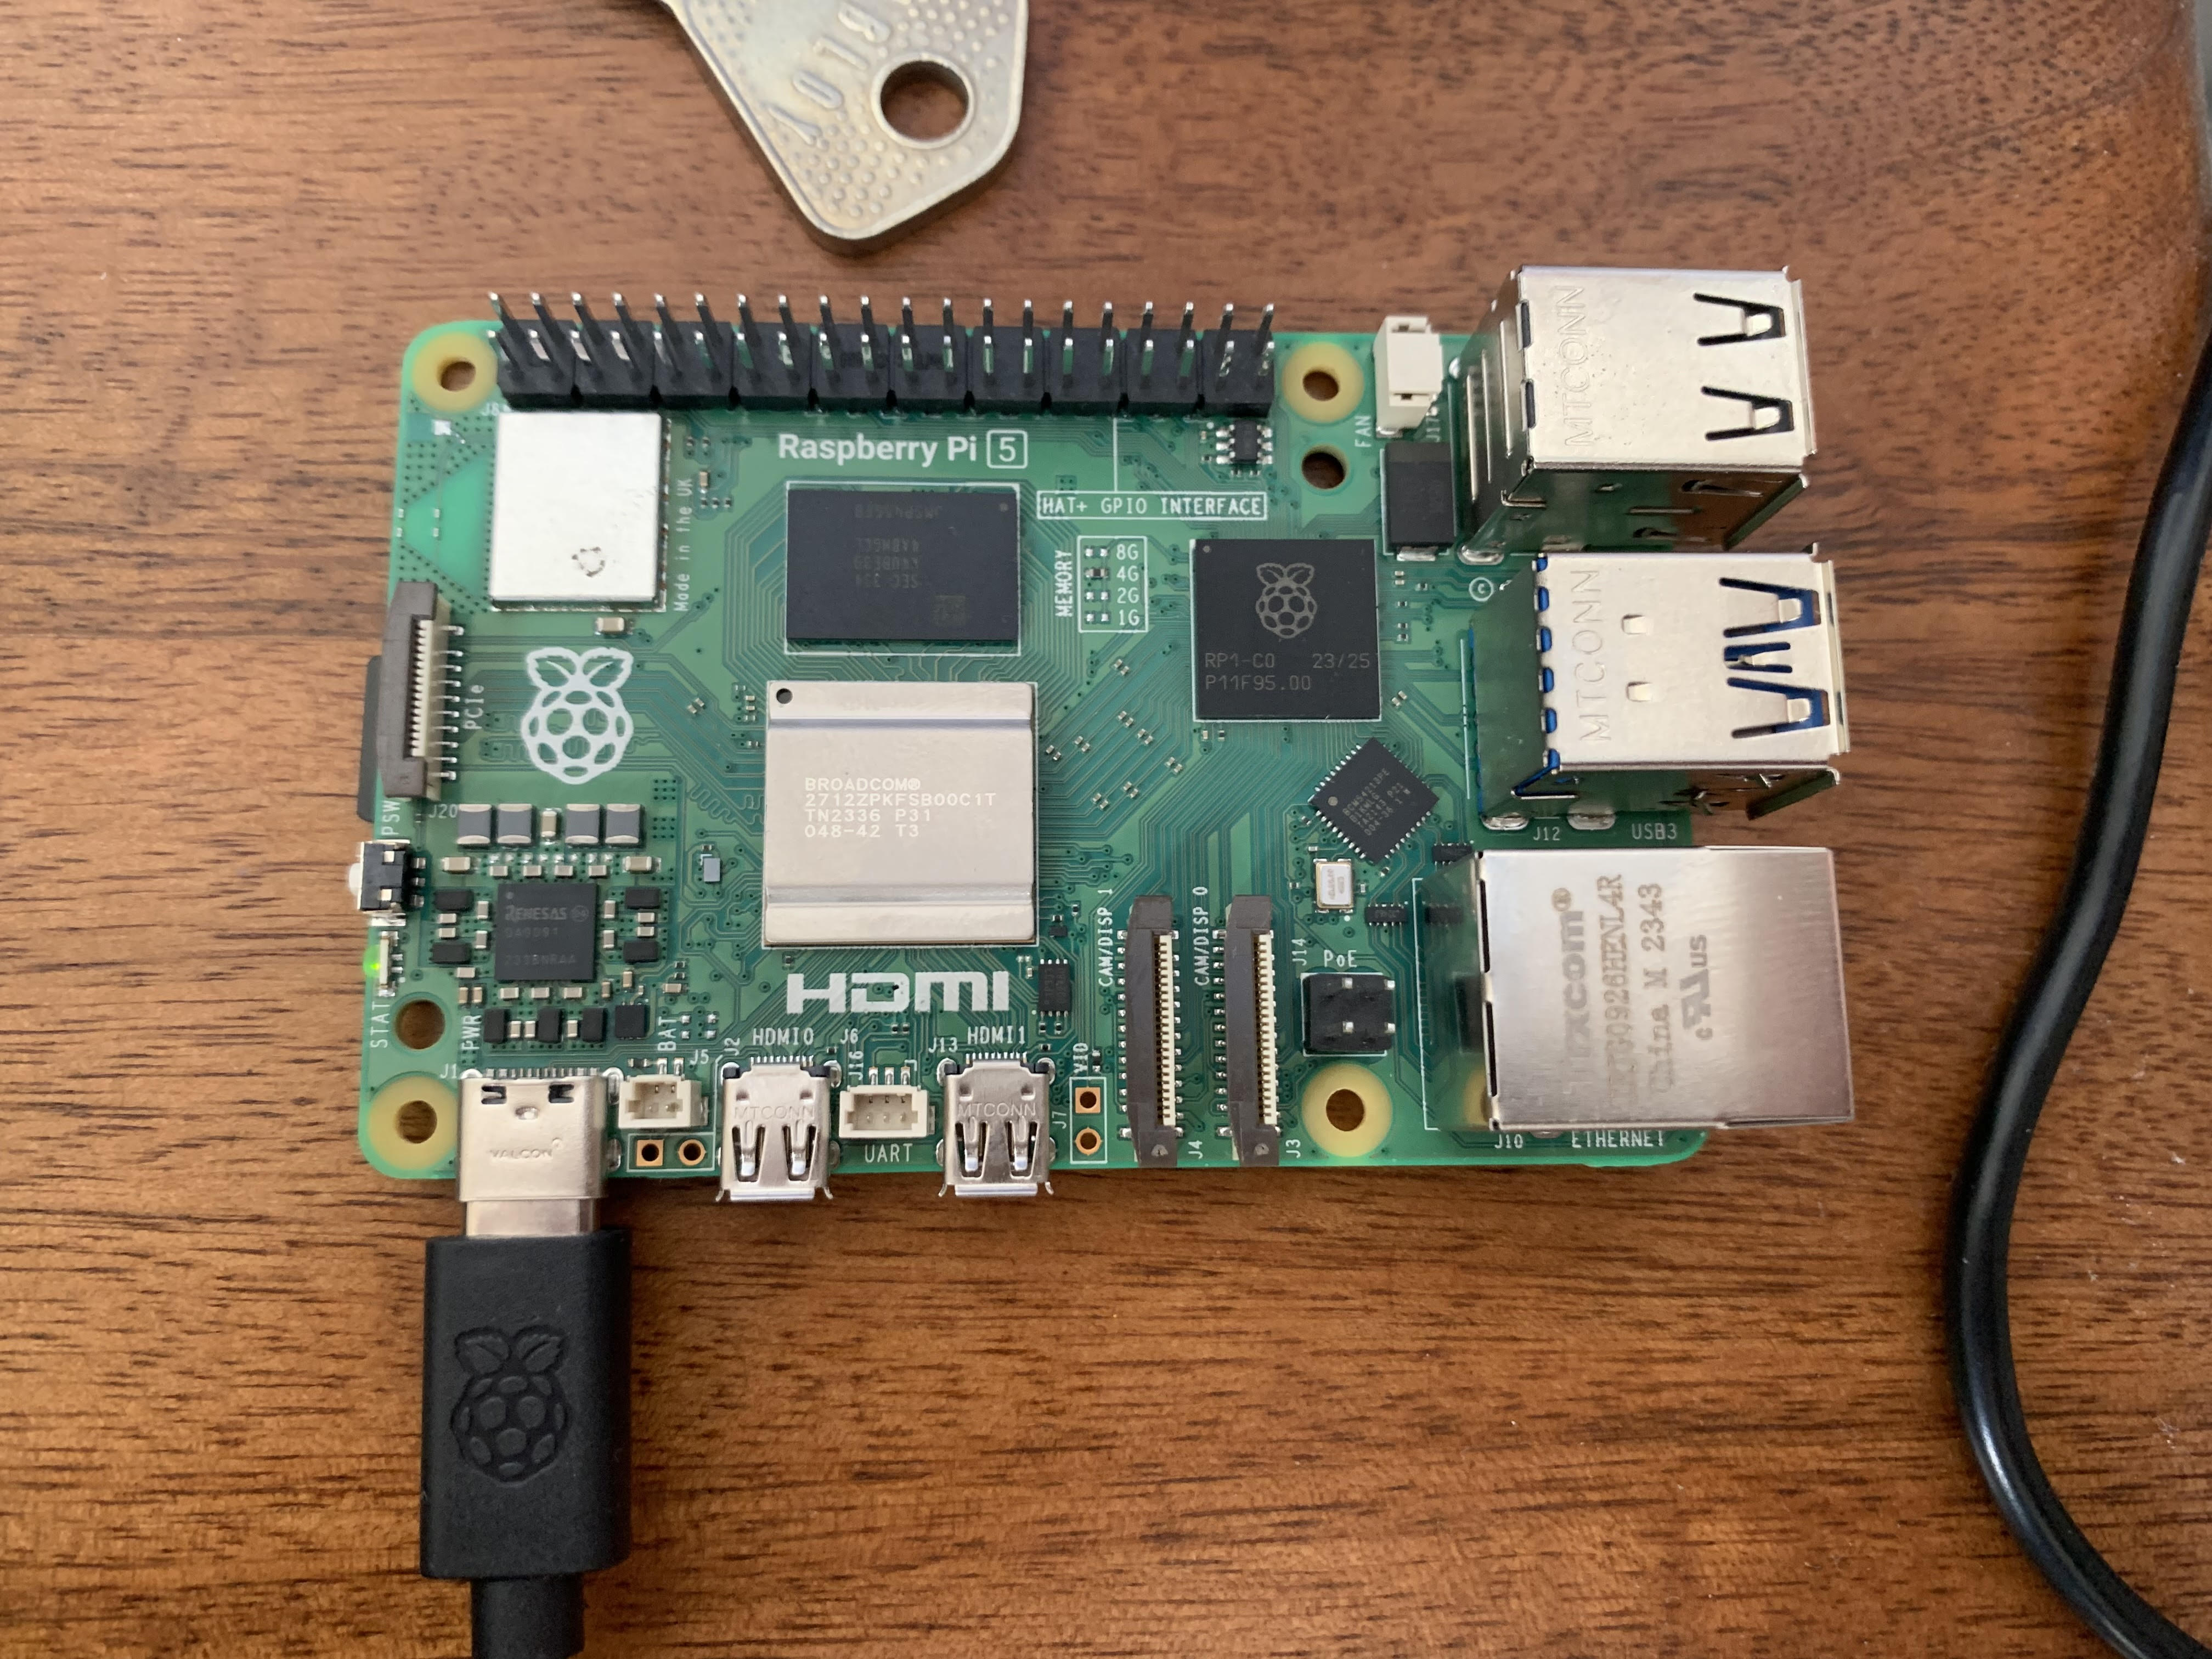
\includegraphics[width=0.5\linewidth]{RasPi5.jpg}
    \caption{Headless Raspberry Pi 5}
    \label{fig:enter-label}
\end{figure}

A similar process was used to remotely control the Israeli VM. This allowed for side-by-side running of tests and comparison of results. 

\begin{figure}
    \centering
    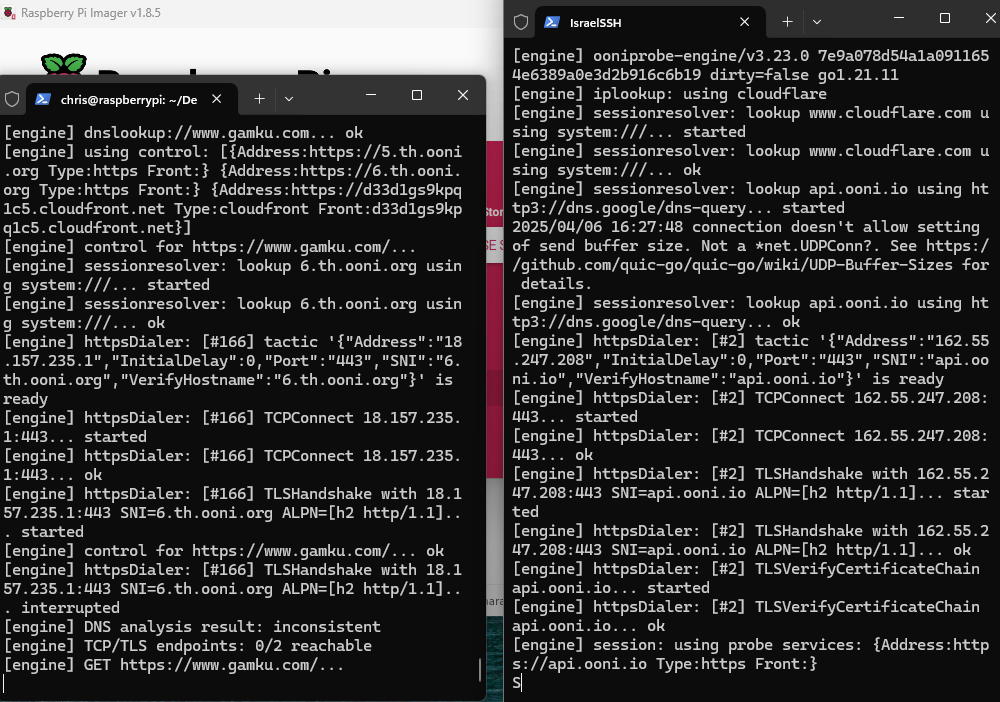
\includegraphics[width=0.5\linewidth]{RunningTestsSideBySideSSH.png}
    \caption{Running OONI tests over SSH}
    \label{fig:enter-label}
\end{figure}

\subsection{Description of Tests Conducted}
Below is a description of the various tests ran by the OONI probe CLI as standard. 
\textbf{Web Connectivity Test}
\textbf{Circumvention Test}
\textbf{Instant Messaging Test}
\textbf{Middlebox Test}
\textbf{my-websites.txt}



\section{Privacy \& Security Concerns}
The following section contains information on privacy and security concerns associated with the completion of the dissertation. This was completed in conjuncture with an assignment given in the CSU44302 Security and Privacy module. 
In writing a dissertation, it is crucial to consider the potential impacts of the research. This document discusses the security and privacy concerns associated with researching internet censorship. Initially, theoretical vulnerabilities will be explored. Specific cases such as Israel and Ireland will then be analyzed. Finally, a practical perspective will examine realistic security and privacy concerns, along with relevant case studies.

\subsection{OONI Probe}
OONI's positive track record is emphasized by the claim: \textit{“To our knowledge, no OONI Probe user has ever faced consequences as a result of using our software.”} \cite{OONIRisks}. The success of OONI is critically dependent on users conducting tests without repercussions. However, OONI outlines several scenarios in which running their probe may be unwise. This includes users residing in countries with a history of prosecuting similar activities, surveillance concerns, or legal restrictions on accessing content. Users who fall into one or more of these categories should be wary of the potential risks. In this context, operating in Ireland with no reason to believe I am under surveillance, I am considered a low-risk user.

\subsection{SSH \& Virtual Machine}
A virtual machine (VM) emulates a computer system. It is a file (.img) that contains instructions to create a virtual environment, leveraging physical PC resources. The provider was chosen based on location availability, with Interhost offering a machine in Tel Aviv. The shared nature of resources introduces vulnerabilities. The number of users sharing the same hardware is unknown, so file-sharing precautions were taken. Storing sensitive information on this VM may be unwise for these reasons.

SSH is a cryptographic protocol that allows users to securely and remotely control a machine over an unsecured network. It employs a client-server model with public-private key pairs for encryption and password authentication. In this project, SSH was used to remotely control the VM in Tel Aviv. Upon generating key pairs, authentication was established, and the VM became accessible. Provided secure settings are maintained and the private key is never shared, SSH is a reliable and trustworthy protocol \cite{SSHManual}.

\subsection{Other Security and Privacy Considerations}
Personal safety risks in researching internet censorship must be addressed. My supervisor highlighted that selecting a comparison country required more than just finding a contrast. Publishing documents that critique government censorship has historically been risky \cite{JulianAssange, EdwardSnowden}. However, this research is relatively low-risk. Particularly compared to cases like Assange or Snowden. MIFTAH, an organization advocating open dialogue on the Israel-Palestine conflict, reported 310 press freedom violations from 2000-2003 \cite{MIFTAHReport2003}. Although Israel has a history of reprisals, these incidents were tied to conflict zones such as Gaza. This research is not of a whistleblowing nature, reducing potential risks.

Researching Israeli state-sponsored internet censorship inevitably intersects with ongoing conflicts. The thesis remains unbiased and non-political. Historical events are included only to provide accurate context for internet censorship analysis. While Israel’s military has strong ties to information control \cite{IsraelCensorship}, it is crucial that internet censorship is examined from an empirical lense.

The security and privacy considerations for this project required assessing all tools used. OONI’s privacy and security protocols appear robust. Its strong track record reinforces this confidence. SSH, as a long-established protocol, remains secure when best practices are followed. Potential consequences of researching this area are more extensive than initially anticipated. However, given my threat model, adverse effects are unlikely. Best practices will continue to be followed to ensure nonpartisan, data-driven research.